\documentclass[11pt]{article}
\usepackage[margin=1in]{geometry}
\usepackage[T1]{fontenc}
\usepackage{mathptmx}
\usepackage{setspace}\setstretch{1.02}
\usepackage{booktabs,xspace,graphicx,caption}
\usepackage{enumitem}\setlist{itemsep=2pt,topsep=4pt,parsep=0pt}
\captionsetup{font=footnotesize,labelfont=bf,skip=4pt}
\usepackage[hidelinks]{hyperref}
\usepackage{natbib}\bibpunct{(}{)}{;}{a}{}{,}
\xspaceaddexceptions{\%}
% generated by scripts/17_numbers.py -- do not edit
\newcommand{\NfirmYears}{34,333\xspace}
\newcommand{\Nfirms}{4,078\xspace}
\newcommand{\NlinkedFirms}{11,182\xspace}
\newcommand{\CorrHeadcount}{0.89\xspace}
\newcommand{\GitHubValid}{2.6\xspace}
\newcommand{\HFValid}{20\xspace}
\newcommand{\GenAIrows}{3.9\xspace}
\newcommand{\HoneB}{1.21\xspace}
\newcommand{\HoneT}{9.7\xspace}
\newcommand{\HonePct}{3.3\xspace}
\newcommand{\HoneIndB}{0.74\xspace}
\newcommand{\HoneIndT}{3.2\xspace}
\newcommand{\EntryAloneB}{-0.28\xspace}
\newcommand{\EntryAloneT}{-3.3\xspace}
\newcommand{\EntryAloneAbs}{0.28\xspace}
\newcommand{\PkgHoneB}{-1.08\xspace}
\newcommand{\PkgHoneT}{10.6\xspace}
\newcommand{\PkgHoneAbs}{1.08\xspace}
\newcommand{\PkgPyrB}{-0.35\xspace}
\newcommand{\PkgPyrT}{5.6\xspace}
\newcommand{\PkgRemB}{-0.31\xspace}
\newcommand{\PkgRemT}{4.6\xspace}
\newcommand{\PkgAgeB}{0.13\xspace}
\newcommand{\PkgAgeT}{2.6\xspace}
\newcommand{\PyrHi}{13.5\xspace}
\newcommand{\PyrLo}{6.9\xspace}
\newcommand{\RemHi}{13.2\xspace}
\newcommand{\RemLo}{7.3\xspace}
\newcommand{\AgeHi}{9.0\xspace}
\newcommand{\AgeLo}{11.5\xspace}
\newcommand{\FSF}{562\xspace}
\newcommand{\FSB}{0.18\xspace}
\newcommand{\IVtiltB}{6.5\xspace}
\newcommand{\IVtiltSE}{0.7\xspace}
\newcommand{\PretrendP}{0.011\xspace}
\newcommand{\Mbar}{1.5\xspace}
\newcommand{\TrendB}{1.38\xspace}
\newcommand{\TrendBT}{10.2\xspace}
\newcommand{\LateB}{1.26\xspace}
\newcommand{\LateBT}{10.2\xspace}
\newcommand{\NegCtl}{-0.44\xspace}
\newcommand{\NegCtlT}{3.6\xspace}
\newcommand{\PlaceboNineteen}{-0.26\xspace}
\newcommand{\PlaceboNineteenT}{2.7\xspace}
\newcommand{\EvTwentyThree}{1.25\xspace}
\newcommand{\EvTwentyFive}{1.80\xspace}
\newcommand{\ModelsToFirstU}{3,483\xspace}
\newcommand{\ModelsU}{4,156\xspace}
\newcommand{\ModelsToFirstFree}{12\xspace}
\newcommand{\ShareHoneSig}{54\xspace}
\newcommand{\HoneMaxT}{12.1\xspace}
\newcommand{\NbaseSpecs}{648\xspace}
\newcommand{\BonfCrit}{4.2\xspace}
\newcommand{\GuardExploreSuccess}{no\xspace}
\newcommand{\GuardConfHoneT}{7.4\xspace}
\newcommand{\Bnull}{1,000\xspace}
\newcommand{\PotemU}{26.5\xspace}
\newcommand{\PotemFree}{93.4\xspace}
\newcommand{\PotemBonf}{0.0\xspace}
\newcommand{\PotemSpec}{3.3\xspace}
\newcommand{\PotemNWC}{5.0\xspace}
\newcommand{\PotemGuard}{0.6\xspace}
\newcommand{\BGuard}{500\xspace}
\newcommand{\GuardHonePot}{48\xspace}
\newcommand{\pNWChOne}{0.001\xspace}
\newcommand{\pNWCpkg}{0.056\xspace}
\newcommand{\NullHoneQ}{8.6\xspace}
\newcommand{\NullHoneMed}{7.4\xspace}
\newcommand{\BonfHoneCrit}{3.8\xspace}
\newcommand{\BonfHonePot}{100\xspace}
\newcommand{\NullShareHoneSig}{34\xspace}
\newcommand{\pBPyr}{0.002\xspace}
\newcommand{\BBPyr}{500\xspace}
\newcommand{\SelPyr}{0.4\xspace}
\newcommand{\HolmPyr}{0.006\xspace}
\newcommand{\pBRem}{0.046\xspace}
\newcommand{\BBRem}{500\xspace}
\newcommand{\SelRem}{92.8\xspace}
\newcommand{\HolmRem}{0.092\xspace}
\newcommand{\pBAge}{0.313\xspace}
\newcommand{\BBAge}{500\xspace}
\newcommand{\SelAge}{76.6\xspace}
\newcommand{\HolmAge}{0.313\xspace}
\newcommand{\PlantPowerLow}{98\xspace}
\newcommand{\PlantPowerMid}{98\xspace}
\newcommand{\PlantPowerHigh}{98\xspace}
\newcommand{\PlantPowerBonf}{93\xspace}
\newcommand{\PlantPowerU}{100\xspace}
\newcommand{\WinnerCurse}{3.2\xspace}
\newcommand{\MCsizeNWC}{5.0\xspace}
\newcommand{\MCsizeNWCpkg}{0.0\xspace}
\newcommand{\MCsizeU}{0.0\xspace}
\newcommand{\MCsizeSpec}{11.0\xspace}
\newcommand{\MCsizeLeak}{10.3\xspace}
\newcommand{\MCsizeLeakReplay}{5.0\xspace}
\newcommand{\MCsizeConf}{90.0\xspace}
\newcommand{\MCpowerNWChOne}{100.0\xspace}
\newcommand{\MCpowerNWC}{82.0\xspace}
\newcommand{\MCpowerU}{82.0\xspace}
\newcommand{\MCR}{300\xspace}
\newcommand{\MCB}{39\xspace}
\newcommand{\RegistryHash}{9aec7d8707aa63a2\xspace}
\newcommand{\RegistryTime}{2026-09-29 04:19:18 BST\xspace}

% generated by scripts/25_aggregate_validity.py -- do not edit
\newcommand{\VSelPyr}{0.4\xspace}
\newcommand{\VNselPyr}{2\xspace}
\newcommand{\VpSelPyr}{0.002\xspace}
\newcommand{\VpFreePyr}{0.002\xspace}
\newcommand{\VpFixPyr}{0.002\xspace}
\newcommand{\VFreeObsPyr}{6.3\xspace}
\newcommand{\VpResSelPyr}{0.002\xspace}
\newcommand{\VpResFreePyr}{0.002\xspace}
\newcommand{\VpResFixPyr}{0.002\xspace}
\newcommand{\VResHolmTenPyr}{0.020\xspace}
\newcommand{\VpFLSelPyr}{0.002\xspace}
\newcommand{\VpFLFreePyr}{0.002\xspace}
\newcommand{\VpFLFixPyr}{0.002\xspace}
\newcommand{\VFLHolmTenPyr}{0.020\xspace}
\newcommand{\VHolmThreePyr}{0.006\xspace}
\newcommand{\VHolmTenPyr}{0.020\xspace}
\newcommand{\VMinPPyr}{0.010\xspace}
\newcommand{\VMaxTPyr}{0.171\xspace}
\newcommand{\VMinPFreePyr}{0.009\xspace}
\newcommand{\VSelRem}{92.8\xspace}
\newcommand{\VNselRem}{464\xspace}
\newcommand{\VpSelRem}{0.046\xspace}
\newcommand{\VpFreeRem}{0.601\xspace}
\newcommand{\VpFixRem}{0.018\xspace}
\newcommand{\VFreeObsRem}{14.8\xspace}
\newcommand{\VpResSelRem}{0.054\xspace}
\newcommand{\VpResFreeRem}{0.337\xspace}
\newcommand{\VpResFixRem}{0.058\xspace}
\newcommand{\VResHolmTenRem}{0.485\xspace}
\newcommand{\VpFLSelRem}{0.032\xspace}
\newcommand{\VpFLFreeRem}{0.693\xspace}
\newcommand{\VpFLFixRem}{0.184\xspace}
\newcommand{\VFLHolmTenRem}{0.287\xspace}
\newcommand{\VHolmThreeRem}{0.092\xspace}
\newcommand{\VHolmTenRem}{0.413\xspace}
\newcommand{\VMinPRem}{0.678\xspace}
\newcommand{\VMaxTRem}{0.279\xspace}
\newcommand{\VMinPFreeRem}{0.979\xspace}
\newcommand{\VSelAge}{76.6\xspace}
\newcommand{\VNselAge}{383\xspace}
\newcommand{\VpSelAge}{0.313\xspace}
\newcommand{\VpFreeAge}{0.002\xspace}
\newcommand{\VpFixAge}{0.022\xspace}
\newcommand{\VFreeObsAge}{7.0\xspace}
\newcommand{\VpResSelAge}{0.234\xspace}
\newcommand{\VpResFreeAge}{0.004\xspace}
\newcommand{\VpResFixAge}{0.228\xspace}
\newcommand{\VResHolmTenAge}{1.000\xspace}
\newcommand{\VpFLSelAge}{0.365\xspace}
\newcommand{\VpFLFreeAge}{0.220\xspace}
\newcommand{\VpFLFixAge}{0.146\xspace}
\newcommand{\VFLHolmTenAge}{1.000\xspace}
\newcommand{\VHolmThreeAge}{0.313\xspace}
\newcommand{\VHolmTenAge}{1.000\xspace}
\newcommand{\VMinPAge}{0.678\xspace}
\newcommand{\VMaxTAge}{0.651\xspace}
\newcommand{\VMinPFreeAge}{0.009\xspace}
\newcommand{\VBjoint}{1,000\xspace}
\newcommand{\VJointSuccess}{94.0\xspace}
\newcommand{\VFwerUnadj}{34.9\xspace}
\newcommand{\VFwerHolmThree}{14.4\xspace}
\newcommand{\VFwerHolmTen}{4.7\xspace}
\newcommand{\VBcovA}{1,000\xspace}
\newcommand{\VcovAph}{0.001\xspace}
\newcommand{\VcovApkg}{0.137\xspace}
\newcommand{\VcovAPotU}{40.3\xspace}
\newcommand{\VcovAPotFree}{100.0\xspace}
\newcommand{\VcovAhQ}{8.0\xspace}
\newcommand{\VcovAhMax}{9.3\xspace}
\newcommand{\VcovARsq}{53\xspace}
\newcommand{\VTypeAhMax}{9.8\xspace}
\newcommand{\VcorrExpRem}{0.62\xspace}
\newcommand{\VcorrExpPyr}{$-$0.53\xspace}
\newcommand{\VcorrExpAI}{0.49\xspace}
\newcommand{\VcorrExpGrowth}{0.16\xspace}
\newcommand{\VcorrPyrRemCell}{$-$0.38\xspace}
\newcommand{\VcorrPyrWageCell}{$-$0.33\xspace}
\newcommand{\VcorrPyrIlmCell}{0.26\xspace}
\newcommand{\VpTmax}{0.124\xspace}
\newcommand{\VSecWorld}{2.5\xspace}
\newcommand{\VSpeedup}{72\xspace}
\newcommand{\VFitsWorld}{5,647\xspace}
\newcommand{\VPyfixestWorld}{182\xspace}
\newcommand{\VPyfixestModel}{0.032\xspace}
\newcommand{\VNhPass}{347\xspace}
\newcommand{\VExSingleNull}{17.0\xspace}
\newcommand{\VExNaiveNull}{19.5\xspace}
\newcommand{\VBudUThousand}{3.7\xspace}
\newcommand{\VBudUReal}{25.7\xspace}
\newcommand{\VBudFreeTwelve}{8.3\xspace}
\newcommand{\VBudFreeHundred}{23.5\xspace}
\newcommand{\VBudUTwelve}{0.9\xspace}
\newcommand{\VModelsMin}{2,169\xspace}
\newcommand{\VModelsMax}{5,171\xspace}
\newcommand{\VModelsMed}{2,790\xspace}
\newcommand{\VTriples}{21\xspace}
\newcommand{\VBaseDistinct}{53\xspace}
\newcommand{\VExNull}{6.5\xspace}
\newcommand{\VExLevel}{6.0\xspace}
\newcommand{\VExCovMax}{7.5\xspace}
\newcommand{\VExStratMax}{45.0\xspace}
\newcommand{\VExNcells}{12\xspace}
\newcommand{\VExNWCSixTen}{100.0\xspace}
\newcommand{\VExSingleSixTen}{84.5\xspace}
\newcommand{\VExNaiveSixTen}{87.0\xspace}
\newcommand{\VExCovSixTen}{5.5\xspace}
\newcommand{\VExStratSixTen}{19.5\xspace}
\newcommand{\VExSpurSixTen}{26\xspace}
\newcommand{\VExNWCSixTwenty}{100.0\xspace}
\newcommand{\VExSingleSixTwenty}{100.0\xspace}
\newcommand{\VExNaiveSixTwenty}{100.0\xspace}
\newcommand{\VExCovSixTwenty}{4.5\xspace}
\newcommand{\VExStratSixTwenty}{45.0\xspace}
\newcommand{\VExSpurSixTwenty}{51\xspace}
\newcommand{\VExNWCTwoQuarter}{11.5\xspace}
\newcommand{\VExSingleTwoQuarter}{20.0\xspace}
\newcommand{\VExNaiveTwoQuarter}{23.5\xspace}
\newcommand{\VExCovTwoQuarter}{6.5\xspace}
\newcommand{\VExStratTwoQuarter}{6.0\xspace}
\newcommand{\VExSpurTwoQuarter}{3\xspace}
\newcommand{\VExNWCFourFive}{43.0\xspace}
\newcommand{\VExSingleFourFive}{35.0\xspace}
\newcommand{\VExNaiveFourFive}{43.0\xspace}
\newcommand{\VExCovFourFive}{7.0\xspace}
\newcommand{\VExStratFourFive}{8.0\xspace}
\newcommand{\VExSpurFourFive}{9\xspace}
\newcommand{\VExNWCTwoFive}{19.5\xspace}
\newcommand{\VExSingleTwoFive}{25.0\xspace}
\newcommand{\VExNaiveTwoFive}{30.0\xspace}
\newcommand{\VExCovTwoFive}{7.0\xspace}
\newcommand{\VExStratTwoFive}{6.0\xspace}
\newcommand{\VExSpurTwoFive}{5\xspace}
\newcommand{\VMmPermFreeClean}{4.0\xspace}
\newcommand{\VMmPermFixClean}{4.0\xspace}
\newcommand{\VMmResFreeClean}{7.0\xspace}
\newcommand{\VMmResFixClean}{5.0\xspace}
\newcommand{\VMmFLFreeClean}{0.5\xspace}
\newcommand{\VMmFLFixClean}{0.5\xspace}
\newcommand{\VMmNomFixClean}{2.5\xspace}
\newcommand{\VMmNomFreeClean}{4.5\xspace}
\newcommand{\VMmPermFreeTrend}{1.5\xspace}
\newcommand{\VMmPermFixTrend}{2.0\xspace}
\newcommand{\VMmResFreeTrend}{5.5\xspace}
\newcommand{\VMmResFixTrend}{5.0\xspace}
\newcommand{\VMmFLFreeTrend}{1.0\xspace}
\newcommand{\VMmFLFixTrend}{0.5\xspace}
\newcommand{\VMmNomFixTrend}{2.5\xspace}
\newcommand{\VMmNomFreeTrend}{3.5\xspace}
\newcommand{\VMmPermFreeProxy}{65.5\xspace}
\newcommand{\VMmPermFixProxy}{67.5\xspace}
\newcommand{\VMmResFreeProxy}{5.0\xspace}
\newcommand{\VMmResFixProxy}{5.0\xspace}
\newcommand{\VMmFLFreeProxy}{0.5\xspace}
\newcommand{\VMmFLFixProxy}{0.5\xspace}
\newcommand{\VMmNomFixProxy}{95.0\xspace}
\newcommand{\VMmNomFreeProxy}{96.0\xspace}
\newcommand{\VMmPermFreeNonlin}{35.5\xspace}
\newcommand{\VMmPermFixNonlin}{35.0\xspace}
\newcommand{\VMmResFreeNonlin}{5.5\xspace}
\newcommand{\VMmResFixNonlin}{6.0\xspace}
\newcommand{\VMmFLFreeNonlin}{0.5\xspace}
\newcommand{\VMmFLFixNonlin}{0.5\xspace}
\newcommand{\VMmNomFixNonlin}{96.0\xspace}
\newcommand{\VMmNomFreeNonlin}{96.5\xspace}
\newcommand{\VMmPermFreeAll}{91.5\xspace}
\newcommand{\VMmPermFixAll}{95.0\xspace}
\newcommand{\VMmResFreeAll}{4.5\xspace}
\newcommand{\VMmResFixAll}{4.5\xspace}
\newcommand{\VMmFLFreeAll}{0.5\xspace}
\newcommand{\VMmFLFixAll}{0.5\xspace}
\newcommand{\VMmNomFixAll}{100.0\xspace}
\newcommand{\VMmNomFreeAll}{96.5\xspace}

\title{\textbf{Potemkin Findings: Calibrating AI Research Loops with Null Worlds}\\[3pt]
\large Stage 1 proposal --- \textit{Organization Science} special issue ``AI-Enabled Frontiers in Organizational Science''}
\date{}
\begin{document}
\maketitle
\vspace{-2em}

\section*{Executive summary: The contribution in one sentence}
We can trust what an AI research loop finds only if we know how often it would ``find'' the same thing when nothing is
there. We build tools that measure this on firm data by rerunning the loop's whole search
on shuffled copies of the data in which the true effect is zero. The result is a valid error rate if every choice made after seeing results is rerun and the shuffle is fair. In our application, an
unchecked loop reports four significant findings at once in \PotemU\% of worlds in which none is true. A technical appendix and a research artifact accompany this proposal.

\section*{Why this matters now}
AI agents can now do the whole empirical part of organizational research: they propose ideas, assemble data, run models,
and revise until the hypotheses ``work.'' Gartenberg et al.\ (2026) report that submissions to this journal rose 42\%
after ChatGPT while writing quality fell. The special issue asks
whether AI research loops produce valid social science or ``Potemkin villages of slop,'' impressive fronts with nothing
behind them.

A loop is a procedure, and every procedure has an error rate, namely how often it reports a
finding that is not real. What has been missing is a practical way to measure that rate for a loop that changes course as it sees
results, and to build the search into the $p$-values it reports.

The problem is sharpest in organization science. A typical study claims a main effect and the conditions that make it
stronger or weaker, on yearly firm data in which each concept has several reasonable measures. Every measure, control
set, sample rule, and condition is a fork in the road; scholars have long worried about the resulting ``search for
asterisks'' (Bettis 2012). An AI loop makes that search
free and invisible.

\section*{How Null-World Calibration works}
We test a loop the way one tests a smoke alarm, by checking whether it goes off when there is no fire. We run the loop on many copies of the data with no effect (\emph{null worlds}) and count how often it still reports
success.
\begin{enumerate}
\item \textbf{Freeze.} Before any result exists, every choice the loop may make (measures, controls, samples, and
moderators with their predicted directions) and its search rules are written to a registry and locked with a digital
fingerprint (a hash), so any later change would show.
\item \textbf{Run.} The search runs on the real data as code. It tries one version of the analysis after another and stops
by its own rule, so it can be rerun exactly. Our two coded rules are benchmarks for an agent's search, not
descriptions of how agents behave (Table~\ref{tab:ledger}).
\item \textbf{Replay.} We rerun the search on \Bnull null worlds. Each shuffles which firm had which AI exposure among firms
in the same industry sector and leaves everything else untouched. The shuffle is fair only if, absent an effect, a firm
could equally have had any sector peer's exposure. Within sectors, exposure is correlated with other traits
(\VcorrExpRem with digitizable work), so we test this (Key risks). The share of worlds in which the loop reports success
is its \emph{Potemkin rate}. The share in which it reports a result at least as strong as the real one is a
\emph{search-adjusted $p$-value}, which already accounts for every analysis tried.
\item \textbf{Test.} We then test the mechanisms and boundary conditions that theory predicts. If AI takes over junior
tasks, task-based theory (Autor et al.\ 2003) and the theory of knowledge hierarchies (Garicano 2000) predict a larger
shift to experienced hires where work is already digital or hierarchies are bottom-heavy (mechanisms), because
technology takes over codifiable tasks and a hierarchy solves its routine problems at the bottom. Structural-inertia
theory (Hannan and Freeman 1984) predicts a smaller shift in older firms, whose routines are harder to change (a
boundary condition). Each
is tested with a \emph{moderator}, a firm trait that should strengthen or weaken the effect, by shuffling that trait
among firms of similar sector and exposure. This also breaks the trait's links to other traits, so a small $p$ shows that
the trait matters, not yet that it changes the effect. Two more kinds of worlds separate the two: a \emph{conditional
shuffle} moves only the part of the trait that sector, exposure, and the other traits do not explain, and
\emph{rebuilt-outcome} worlds remove only the trait's effect from the outcomes (Freedman and Lane 1983). The loop picked
three of ten candidate moderators, so we correct for all ten.
\item \textbf{Plant.} Effects of known size are added to null worlds to measure how often the loop finds them (power) and
how much it exaggerates them (the \emph{winner's curse}).
\end{enumerate}
Figure~\ref{fig:steps} follows the five steps through our application.

\begin{figure}[t]\centering
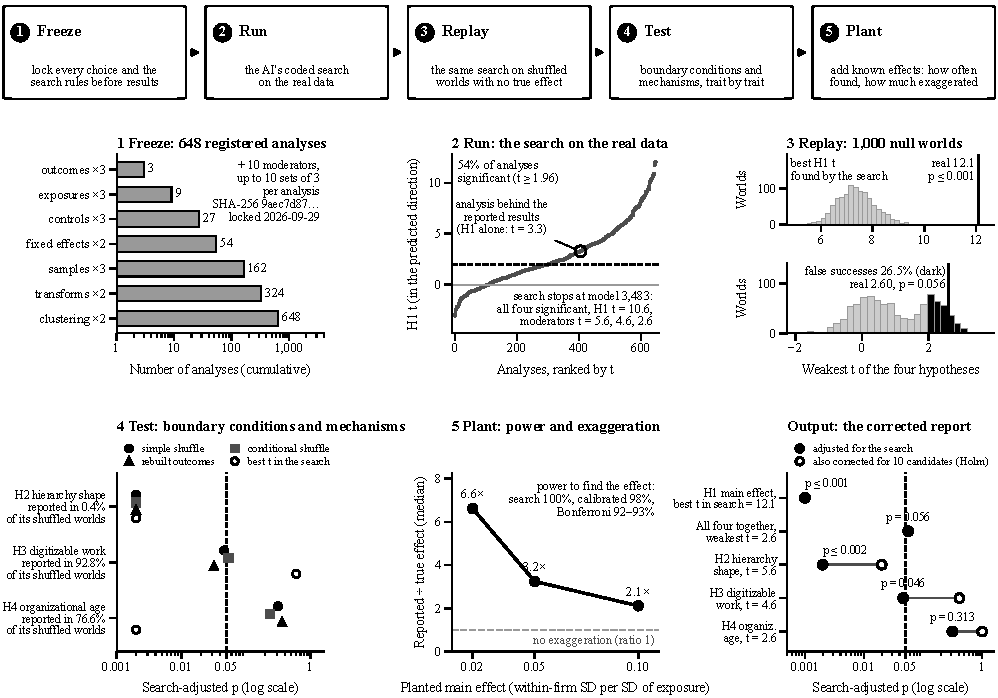
\includegraphics[width=0.96\linewidth]{../figures/fig6_steps.pdf}
\caption{\textbf{Null-World Calibration step by step, on the application.} (1)~The locked registry: \NbaseSpecs versions
of the analysis, each able to add up to ten sets of three moderators. (2)~The main-effect (H1) $t$ of each version on the
real data; the search first found all four hypotheses significant after \ModelsToFirstU models. (3)~Null worlds: the best
H1 $t$ the search found (top) and the weakest $t$ of the four hypotheses (bottom); lines mark the real values; dark bars
are false successes. (4)~Each boundary condition or mechanism's search-adjusted $p$ under a simple shuffle (circles), a
conditional shuffle (squares), and rebuilt outcomes (triangles). A world in which the trait is not reported counts as
weaker than the real data, so these $p$ reflect strength and selection; open circles use the trait's best $t$ in the
search, defined in every world. (5)~Planted effects: reported over true size. (Output)~Each result with its own
search-adjusted $p$, and the correction for ten candidates (open; Holm). Dashed line: 0.05.}
\label{fig:steps}
\end{figure}

\section*{What we have done}
\begin{enumerate}
\item \textbf{What is new, and what is not.} The guarantee is classical. A shuffle test is exact for any result produced by
a rule fixed before the data are seen, and a search frozen as code is such a rule (Technical Appendix, Theorem~1; Lehmann
and Romano 2022). Existing corrections for trying many models need the list of models fixed in advance (White 2000;
Romano and Wolf 2005), but a loop's list is not fixed; across null worlds, ours fits \VModelsMin to \VModelsMax models and
reports \VTriples different sets of moderators. Correcting for every model the registry allows is valid but blunt
($p=\VpTmax$, against $p=\pNWCpkg$ when the actual stopping rule is replayed). We contribute four things that
make it usable for AI loops: (i)~a replay protocol, under which every choice made after seeing data is code and all else
is locked beforehand; (ii)~null worlds that keep the structure of firm data; (iii)~measures that fixed-list corrections
do not give, namely the Potemkin rate of a whole set of findings, risk by the number of models tried, and the winner's
curse; and (iv)~the open-source Python package \emph{nullworld}, whose engine matches a standard package to
within $10^{-15}$ and reruns the full loop in \VSecWorld seconds (\VSpeedup times faster).

\item \textbf{Who decided what.} The AI agent proposed the registry from the literature, built the data, and wrote the loop; the authors
approved the registry before any outcome was computed. Coded rules made every choice during the run (Table~\ref{tab:ledger}). Rule U pursues the registered hypotheses until they work; U-free may also flip a moderator's
predicted direction after seeing results, as a researcher might explain away a surprise. In null worlds, U reports four significant
findings within 1,000 models in \VBudUThousand\% of worlds and within the \ModelsToFirstU it used on the real data in
\VBudUReal\%; U-free does so within 12 models in \VBudFreeTwelve\%.

\begin{table}[t]\centering\footnotesize
\caption{Who took which decision in the prototype}\label{tab:ledger}
\setlength{\tabcolsep}{5pt}\begin{tabular}{lll}
\toprule
Decision & Taken by & In calibration \\
\midrule
Research question and data & Authors & Fixed, outside the loop \\
Registry (concepts, measures, 10 moderators, search rules) & AI agent; approved by authors & Frozen, locked before results \\
Data assembly, checks, loop code & AI agent; reviewed by authors & Fixed code \\
Choices during the search (next model, moderators, stop) & Coded rule (Stage 2: live agent) & Replayed in every world \\
\bottomrule
\end{tabular}
\end{table}

\item \textbf{A demanding test case.} Did generative AI lead firms to hire fewer beginners and more experienced workers?
We linked r\'esum\'e-based job and skill records to company financial data (Compustat), covering \NfirmYears firm-years at
\Nfirms firms from 2016 to 2025. We compare firms whose work in 2019--2021 was more or less exposed to language models, before and after
ChatGPT's release (a difference-in-differences design). One standard deviation more exposure
raises the share of experienced hires by \HoneB percentage points ($t=\HoneT$). Year-by-year estimates, fake release
dates, and exposure to other kinds of AI point to a break after 2022 specific to language models. The estimate holds even if
post-2022 trend differences were \Mbar times the largest seen before.

\item \textbf{The diagnostic result.}
\begin{itemize}
\item On the real data, rule U found four significant results after
\ModelsToFirstU models; U-free needed \ModelsToFirstFree. In null worlds, the two rules reported such a set \PotemU\% and
\PotemFree\% of the time.
\item With a split-sample guard (search on half of the firms, check once on the other half), no full set emerged in the search half; the main effect held up in the other half
($t=\GuardConfHoneT$), but only one of its three moderators did.
\item After accounting for the search, the set as a whole is not significant ($p=\pNWCpkg$), but the main effect is
significant, since its best $t$ (\HoneMaxT) beats all \Bnull null worlds ($p\le\pNWChOne$). Of the ten candidate moderators, only hierarchy shape survives the correction for testing ten (Holm
$p=\VHolmTenPyr$; digitizable work \VHolmTenRem, organizational age \VHolmTenAge). Correcting for only the three reported
would confirm one in \VFwerHolmThree\% of worlds in which none of the ten matters. Nor did the loop pick hierarchy
shape by luck, since its best $t$ during the search, defined in every world, is never
beaten in its shuffled worlds ($p\le\VpFreePyr$). Even with all ten moderators shuffled, the loop reports four significant
findings in \VJointSuccess\% of worlds.
\end{itemize}

\item \textbf{Measurement checks an unguarded loop would have missed.} The standard skill label ``GitHub Copilot'' is
correct for only \GitHubValid\% of rows, and a skill's ``first reported'' date tracks when the r\'esum\'e was collected, not
when the skill was adopted.
\end{enumerate}

\section*{What we hope to do in Stage 2}
\begin{enumerate}
\item \textbf{Live-agent loops.} Replace the coded rule with a real AI agent at the same choices (Table~\ref{tab:ledger}), under two
instructions: ``test the registered hypotheses'' and ``find support for
them.'' Each call is logged and repeated in every null world with an open-weight model set to answer the same input the
same way, so the agent's choices are replayed, not frozen. This places real agents on the risk curve between U and
U-free, and measures the cost of letting an agent see results early.
\item \textbf{Concepts measured from text.} Extend null worlds to concepts AI measures from text (earnings calls, job
postings), where measurement and hypothesis choice interact.
\item \textbf{A Potemkin-rate service.} An open tool that returns a calibration report for any registry and replayable loop.
\item \textbf{A many-agent study.} Give several AI agents the same data and question, then calibrate each agent's loop. This
is the AI version of many-analyst studies (Silberzahn et al.\ 2018; Breznau et al.\ 2022).
\end{enumerate}

\paragraph{Timeline.} \textbf{January to mid-February 2027:} live-agent replay and the experiment on seeing results
early. \textbf{By the workshop (19--20 February 2027, Duke University, Fuqua School of Business):} a public release of
the \emph{nullworld} package with documentation and the synthetic data. \textbf{March--April 2027:} text-measured concepts and the
many-agent study. \textbf{May 2027:} the calibration service and the final article.

\section*{Key risks and how we address them}
\begin{itemize}
\item \textbf{Is the shuffle fair?} In simulations, a trait linked to exposure that only raises or lowers a firm's outcomes
overall is harmless (\VExLevel\% false alarms at the 5\% level). A trait that changes outcomes after 2022 creates a false
effect that every test of the exposure--outcome link picks up, calibrated or not. False alarms reach \VExNWCFourFive\% when
that false effect is only \VExSpurFourFive\% of our estimate. If the trait is measured, worlds that keep exposure's link
to it restore the correct rate (at most \VExCovMax\% across \VExNcells settings); on the real data, the main effect beats
all \VBcovA such worlds built on twelve firm traits ($p\le\VcovAph$). Unmeasured traits are left to the design checks.
\item \textbf{Testing boundary conditions and mechanisms.} In simulations where no moderator truly changes the effect, a
moderator's own post-2022 trend is harmless (\VMmPermFixTrend\% false alarms). But a correlated moderator with a real
effect, together with a curved effect of exposure, pushes the simple shuffle to \VMmPermFixAll\%. The conditional shuffle
keeps the correct rate (\VMmResFixAll\%); rebuilt-outcome worlds are cautious (\VMmFLFixAll\%). On the real data,
hierarchy shape survives all three.
\item \textbf{Adoption.} Authors may resist registries. The protocol asks only that inputs that cannot be rerun be frozen
before results are seen, which AI loops make cheap.
\item \textbf{Licensed data.} We cannot post the licensed workforce or Compustat data. Following the call's FAQ, the
research artifact provides a synthetic copy of the data on which the loop and all null worlds can be rerun.
\end{itemize}

\section*{How organizational and social science would change}
AI makes exploring cheap, since an agent can try every path. What stays scarce is knowing which discoveries would have appeared
by chance anyway. If this project succeeds, a manuscript produced with an AI loop would arrive with its locked registry,
its replayable loop, and its Potemkin rate. Editors and reviewers could judge the procedure, not only the prose, weakening the
incentive to flood journals with polished but unchecked findings. This is the move toward ``better, not more'' that
the editors call for (Gartenberg et al.\ 2026).

\section*{Fit with the evaluation criteria}
\begin{center}\small
\begin{tabular}{p{3.2cm}p{11.8cm}}
\toprule
Criterion & Evidence \\
\midrule
Novelty & Exact shuffle tests made usable for AI loops that adapt; error rates for whole searches \\
Feasibility & Working prototype on \NfirmYears firm-years; \Bnull worlds per kind on one workstation \\
Stage of development & Validity conditions proved in the technical appendix; simulations of each failure; real-data application \\
Ethicality & Aggregated, licensed secondary data; no human subjects; full disclosure of AI use \\
Reproducibility & Research artifact with the locked registry, numbered scripts, and synthetic data; verified references \\
Scalability & Cost grows in proportion to the number of worlds; runs in parallel \\
Use and adoption & Drop-in package; a calibration report editors and reviewers can request \\
Frontier expansion & Turns AI's capacity for search into a measurable, accountable property of research \\
\bottomrule
\end{tabular}
\end{center}

\section*{References}
{\small
Autor DH, Levy F, Murnane RJ (2003) The skill content of recent technological change: An empirical exploration. \textit{Quart. J. Econom.} 118(4):1279--1333.\par
Bettis RA (2012) The search for asterisks: Compromised statistical tests and flawed theories. \textit{Strategic Management J.} 33(1):108--113.\par
Breznau N, et al.\ (2022) Observing many researchers using the same data and hypothesis reveals a hidden universe of uncertainty. \textit{Proc. Natl. Acad. Sci. USA} 119(44):e2203150119.\par
Freedman D, Lane D (1983) A nonstochastic interpretation of reported significance levels. \textit{J. Bus. Econom. Statist.} 1(4):292--298.\par
Garicano L (2000) Hierarchies and the organization of knowledge in production. \textit{J. Political Econom.} 108(5):874--904.\par
Gartenberg C, Hasan S, Murray A, Pierce L (2026) More versus better: Artificial intelligence, incentives, and the emerging crisis in peer review. \textit{Organ. Sci.} 37(3):795--812.\par
Hannan MT, Freeman J (1984) Structural inertia and organizational change. \textit{Amer. Sociol. Rev.} 49(2):149--164.\par
Lehmann EL, Romano JP (2022) \textit{Testing Statistical Hypotheses}, 4th ed. (Springer, Cham).\par
Romano JP, Wolf M (2005) Stepwise multiple testing as formalized data snooping. \textit{Econometrica} 73(4):1237--1282.\par
Silberzahn R, et al.\ (2018) Many analysts, one data set: Making transparent how variations in analytic choices affect results. \textit{Adv. Methods Practices Psych. Sci.} 1(3):337--356.\par
White H (2000) A reality check for data snooping. \textit{Econometrica} 68(5):1097--1126.\par
}
\end{document}
